\documentclass[]{article}
\usepackage{natbib}
\usepackage{url}
\usepackage{graphicx}

%opening
\title{}
\author{}

\begin{document}

\maketitle

\begin{abstract}

\end{abstract}

\citet{Annand2020} presented participants with a novel task setup. This setup consists of a stylus on a computer screen controlled by two rotary dials. One dial controlled the $X$-direction of the stylus while the other dial was used to control the $Y$-direction of the stylus. In this, the setup is reminiscent of \textit{Etch A Sketch}, the famous mechanical drawing device \citep{EtchASketch}. Using the setup, participants were instructed to trace out a circle on the computer screen by following a target indicator. The indicator moved along a circular path with a period of either $\sim$5 seconds or  $\sim$2.5 seconds.

Participants' performance in following the target indicator was quantified as a function of the number of trials. With increased practice, participants' errors decreased. More interestingly, \citet{Annand2020} had individual participants or dyads performing the task. When individuals performed the task, participants controlled both dials. Dyads controlled one dial each.

Throughout their paper, \citet{Annand2020} present several hypotheses about how the (relative) performance of dyads and individuals would increase with practice. Their predictions suggest that \citet{Annand2020} have not performed a computational assessment of the task preventing them from appreciating the strategies available to participants. As \citet{Annand2020} conclude that their setup can be \textit{[used] to probe many different hypotheses of interlimb coordination and motor learning}, we think it is essential to provide a computational analysis. This would allow researchers using this task to appreciate which conclusions it allows to draw (and which deductions are erroneous).

\citet{Annand2020} assume that the task requires individuals to reconfigure the pre-existing intrinsic coupling between limbs throughout the task. The authors assume that moving both arms (or hands) in-phase (or anti-phase) is easier than the 90 degrees offset in arm movement required by the task. Indeed, to draw a circle on the screen, the rotation of one dial should lag (or lead) the other one by 90 degrees. Therefore, dyads should not experience this problem and are hypothesized to perform better initially. Thus far, we agree with the interpretation of the task.

However, \citet{Annand2020} make an error when they state that individuals potentially could outperform dyads by reconfiguring the coupling between limbs to maintain a 90-degree offset. Here, \citet{Annand2020} assume that individuals could achieve better performance than dyads by (learning to) fix the movement of the arms with a 90 degree offset. Indeed they state,

\noindent\textit{[G]reater coupling strength [could give] rise to stronger intrinsic coordination dynamics—could, over the course of learning, be harnessed to achieve more rapid stabilization (and hence better performance) of the new [90-degree] coordination pattern.}

This assertion shows that \citet{Annand2020} do not appreciate that the task they present to participants consists of two independent tasks. In other words, there exists an optimal strategy under which the task can be performed perfectly (zero error) that does not require any coupling between the limbs. Therefore, there is no benefit from reconfiguring the coupling between limbs. 

Therefore, the task presented by \citet{Annand2020} can not be used to assess how people reconfigure the coupling between limbs. Indeed, any increase can be either attributed to a change in coupling (from 0/180 degrees to 90 degrees), or, alternatively, to a reduction in coupling. The task does not allow distinguishing between these two alternatives. Therefore, at best, the task can be used to conclude that \textit{something} changes in the coupling of limbs. 

In this letter, we present evidence to support our assessment of the task presented by \citet{Annand2020} in the following form. First, we present a simple computational model showing that the task consists of two decoupled sub-tasks. Second, we reanalysis the data presented by \citet{Annand2020} showing that participants did indeed learn to decouple their limbs. Thirds, we use the computational model to show that coupling the limbs with an offset of 90 degrees is likely to \textit{decrease} performance.

\section{Computational analysis}

In this section, we analyze the task presented by \citet{Annand2020} to show that it consists of two independent tasks. There are multiple ways in which this could be demonstrated. However, as \citet{Annand2020} focus on learning, we show that an agent can perfectly solve the task by learning to decouple both controls.


\begin{figure*}
	\centering
	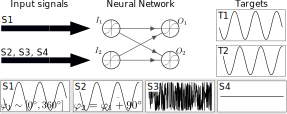
\includegraphics[width=1\linewidth]{neural_network}
	\caption{eqeqeqqqweqeweq}
	\label{fig:neuralnetwork}
\end{figure*}

We use the neural network depicted in figure \ref{fig:neuralnetwork} as a learning agent. The network consists of two input neurons and two output neurons. The neurons have hyperbolic tangent activation functions. The network is trained to produce sinoid output signals $T_1$ and $T_2$ at output neurons $O_1$ and $O_2$, with $T_2$ shifted by 90 degrees with respect to $T_1$.

\begin{figure*}
	\centering
	\includegraphics[width=1\linewidth]{neural_network_0}
	\caption{qweqeqwewqe}
	\label{fig:neuralnetwork0}
\end{figure*}

We trained the neural network to produce the desired output in response to various input signals ($S_1$, $S_2$, $S_3$, and $S4$, figure \ref{fig:neuralnetwork} ). The input signal for neuron $I_1$ is fixed to signal $S_1$, a sinoid wave with a length of 3 periods. Its phase was randomized for each training iteration, i.e., $\varphi_1 \sim [0^\circ, 360^\circ]$.

We varied the input to neuron $I_2$ to demonstrate that the  task of \citet{Annand2020} consists of two independent subtasks. The input to $I_2$ could be either $S_2$, $S_3$, or $S_4$ (figure \ref{fig:neuralnetwork}).

Signal $S_2$ was a sinoid with phase  $ \varphi_2 = \varphi_1 + 90^\circ$. Therefore, when presenting signals $S_1$ and $S_2$ to the neural network as input, we model the task as presented to participants by \citet{Annand2020}: a circular input (target location) has to be converted to a circular output (stylus location). 

Converting $S_1$ and $S_2$ t



    

\bibliographystyle{plainnat}
\bibliography{refs}


\end{document}
